\section{Modularity and extensibility}

\begin{figure}[ht]
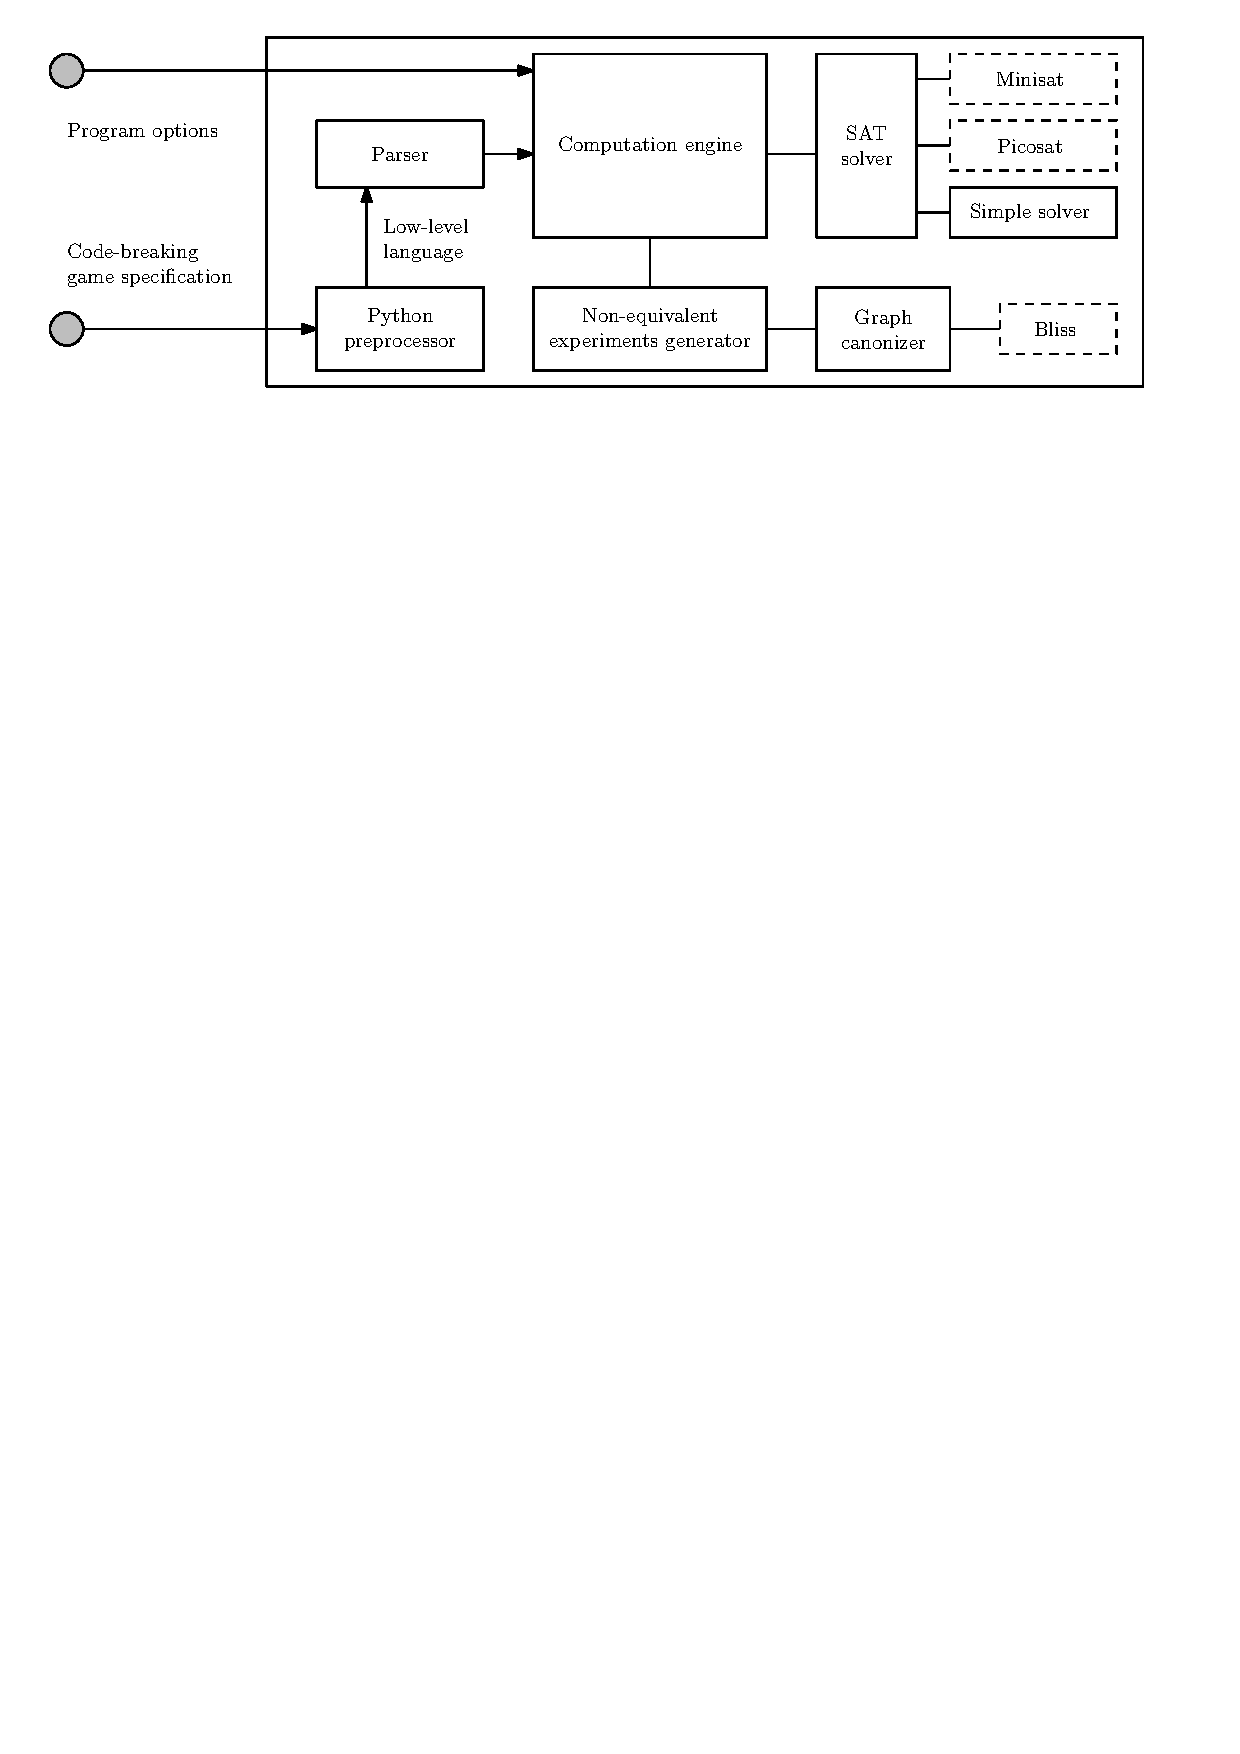
\includegraphics[width=\textwidth]{pictures/modularity.pdf}
\caption{Component diagram of COBRA.}
\label{fig:components}
\end{figure}


COBRA uses external tools for SAT solving and graph canonization.
Nowadays, many high-performance SAT solvers are available
  and multiple tools for graph canonization exists.
COBRA was developed so that other external tools with the same functionality
  can be easily integrated.
\autoref{fig:components} shows a component diagram of
  the modular design of COBRA.

Detailed requirements on a SAT solver and
  on a graph canonization tool are listed in the next sections.

If you want to try another SAT solver, alter the algorithm for model counting,
  or test any other modification,
  you can implement your own solver class that inherits from \texttt{Solver} and
  implements all the necessary methods.

Check the \texttt{solver.h} file and the documentation therein
  for the information about the exact functions required.
Further, you need to to include the file with your class in
  \texttt{main.cpp} and add a new case
  into the \texttt{get\_solver} function in this file.


COBRA can be easily extended with a new strategy or heuristics to selects experiments.
All available strategies are implemented in \texttt{strategy.h/strategy.cpp} file.
If you want to add a new strategy, create a corresponding function in this file
  and add an entry about the strategy
  to the \texttt{breaker\_strategies} table in \texttt{strategy.h}.
A strategy function takes a list of experiments as the only argument
  and returns the index of the selected one.

If the strategy is one-step look-ahead,
  you can use a provided template with a corresponding lambda function.
We demonstrate this possibility with a code snippet of
  the exact implementation of the \emph{exp-models} strategy below.
For exact details, see the documentation in the file.

\begin{lstlisting}[language=C++]
uint breaker::exp_num(vec<Option>& options) {
  return minimize([](Option& o){
    auto models = o.GetNumOfModels();
    int sumsq = 0;
    for (uint i = 0; i < o.type().outcomes().size(); i++) {
      sumsq += models[i] * models[i];
    }
    return (double)sumsq / o.GetTotalNumOfModels();
  }, options);
}
\end{lstlisting}

\section{SAT solving} \label{s:cobra-sat}

COBRA uses a SAT solver for the following tasks.
\begin{itemize}
\item Compute the total number of possible codes.
\item Verify that an experiment is well-formed (see \autoref{s:cobra-modes} for details).
\item Identify satisfiable outcomes of an experiment and disregard the others.
\item Decide whether the game is finished -- whether the accumulated
  knowledge as a formula has only one model.
\item Evaluate the strategies -- count models, fixed variable, etc.
\end{itemize}

Most of these tasks require an \emph{incremental SAT solver}, i.e. a
  sat solver to which you can add constraints and take them back later.
Without this feature, we would have to call the solver from a clean state
  many times on the whole formula, which would ruin the computation time.

COBRA uses a SAT solver as an abstract class, which can have multiple implementations.
This allows a simple extension with another SAT solver.
The solver to be used can be specified with
  the \texttt{-b} or \texttt{--backend} switch.

Solver must implement the following methods:
\begin{itemize}
\item \textsc{AddConstraint}(formula). Adds a constraint to the SAT solver.
\item \textsc{Satisfiable()} $->$ Bool. Decides whether the current formula is satisfiable.
\item \textsc{GetAssignment()} $->$ Assignment.
  After \textsc{Satisfiable} call, this function retrieves
  a satisfying assignment from the solver.
\item \textsc{OpenContext(), CloseContext()}.
  This is our understanding of incremental SAT solving.
  \textsc{OpenContext} adds a context to a stack.
  Every call to \textsc{AddConstraint} adds the constraint to the current context.
  \textsc{CloseContext} removes all the constraint in the current context and removes it
  from the stack. It must be possible to nest contexts arbitrarily.
  The two methods are sometimes called just \textsc{Push} and \textsc{Pop}.
\item \textsc{HasOnlyOneModel()} $->$ Bool. Decides whether to formula has only one model.
  This can be implemented by asking whether the formula is satisfiable,
  if yes, retrieving the satisfying assignment, adding
  a clause with the assignment negated and asking for satisfiability again.
  Adding the new clause should be done in a new context in order not to pollute
  the solver state. The pseudocode is shown in \autoref{alg:onlyonemodel}.

\item \textsc{CountModels()} $->$ Int.
SAT solvers do not typically include support for model counting, the problem
  commonly referred to as \#SAT.
One solution is to use
  special tools designed for this purpose,
  such as SharpSAT\footnote{\url{https://sites.google.com/site/marcthurley/sharpsat}}
  \cite{sharpsat}.
However, these tools do not support incremental solving and
  must be run from a clean state for each formula models of which we want to count.

Second option is to use a SAT solver, repeatedly ask for satisfiability and
  add clauses that forbids the current assignment until we get
  an unsatisfiable formula. The pseudocode is shown in \autoref{alg:modelcounting2}.

Third option is to use a SAT solver and a simple backtracking approach,
  progressively assuming a variable to be true or false and cut the non-perspective
  branches.
The pseudocode is shown as a recursive function in \autoref{alg:modelcounting3}.
\end{itemize}

\begin{algorithm}[ht]
\caption{Decision whether a formula has exactly one model.}
\label{alg:onlyonemodel}
\DontPrintSemicolon
\lIf{not \textsc{Satisfiable()}}{\Return{false}}
$v <- $ \textsc{GetAssignment()}\;
\textsc{OpenContext()}\;
\textsc{AddConstraint($\overline{x_1}\| ... \|\overline{x_n}$)},
  where $\overline{x_i}$ is $\neg\:x_i$ if $v(x_i) = 1$ and $x_i$ otherwise\;
$sat <- $\textsc{Satisfiable()}\;
\textsc{CloseContext()}\;
\Return{$\neg sat$}
\end{algorithm}
\begin{algorithm}[ht]
\caption{Model counting, second option.}
\label{alg:modelcounting2}
\DontPrintSemicolon
$models <- 0$\;
\textsc{OpenContext()}\;
\While{\textsc{Satisfiable()}} {
  $v <- $ \textsc{GetAssignment()}\;
  \textsc{AddConstraint($\overline{x_1}\| ... \|\overline{x_n}$)},
    where $\overline{x_i}$ is $\neg\:x_i$ if $v(x_i) = 1$ and $x_i$ otherwise\;
  $models <- models + 1$\;
}
\textsc{CloseContext()}\;
\Return{$models$}
\end{algorithm}
\begin{algorithm}[h!]
\caption{Model counting, third option.}
\label{alg:modelcounting3}
\DontPrintSemicolon
$models <- 0$\;
$x <- $ any variable from $vars$\;
\textsc{OpenContext()}\;
\textsc{AddConstraint}($x$)\;
\lIf{\textsc{Satisfiable()}}{$models <- models \:+ $ \textsc{count}($vars\setminus \{x\}$)}
\textsc{CloseContext()}\;
\textsc{OpenContext()}\;
\textsc{AddConstraint}($\neg x$)\;
\lIf{\textsc{Satisfiable()}}{$models <- models \:+ $ \textsc{count}($vars\setminus \{x\}$)}
\textsc{CloseContext()}\;
\Return{$models$}
\end{algorithm}

COBRA includes three solver implementations which we describe next.

\subsection{PicoSat}
Picosat\footnote{\url{http://fmv.jku.at/picosat/}} \cite{picosat} is a simple,
  extensible SAT solver, which supports incremental SAT solving exactly in the way
  we need.

Bindings to Picosat are implemented in \texttt{PicoSolver} class.
This class also implements model counting algorithm \ref{alg:modelcounting3}
 as Picosat does not support model counting itself.


\subsection{MiniSat}

Minisat\footnote{\url{http://minisat.se/}} \cite{minisat} is a minimalistic,
  extensible SAT solver that won several SAT competitions in the past.

Minisat does not support incremental SAT solving in the manner we described,
  but it supports assumptions.
You can assume arbitrary number of unit clauses
  (i.e. that a variable is true of false) and ask for satisfiability under
  those assumptions.

The behaviour we want can be simulated by assumptions in the following way.
For each context, we create a new variable, say $a$.
Then, instead of adding clauses $C_1, C_2, ..., C_n$ to the context,
  we add clauses $\{\neg a, C_1\}$, $\{\neg a, C_2\}$, ... $\{\neg a, C_n\}$ and ask
  for satisfiability under the assumption $a$ (in general,
  assumption that all variables of open contexts are true).
Afterwards, when a context is closed, we add a unit clause $\{\neg a\}$,
  which effectively removes all the clauses added in the context.
The only minor issue with this approach is that the variable $a$ is wasted,
  the solver will remember it somewhere and may consume more memory.

Bindings to Minisat are implemented in \texttt{MiniSolver} class.
This class implements the context opening and closing in the way described above
and also model counting algorithm \ref{alg:modelcounting3}.

\subsection{Simple solver}

We include a special SAT solver, called \texttt{SimpleSolver} to show that
  the usage of a proper SAT solver in this application is justifiable.
Simple solver uses another SAT backend (Picosat) to generate all
  models of the initial constraint $\init$ (or of the first constraint, in general).
Later satisfiability questions with additional constraint are
  resolved by going though all possible codes (assignments) and
  checking that the constraints are satisfied.
Model counting and the other functions are implemented similarly.

\subsection{Transformation to CNF}

The input formula for a SAT solver must be typically specified
  in the conjunctive normal form(CNF).
As we do not have such requirement for formulas in the input format,
  and allow non-standard numerical operators,
  we need to transform a formula to CNF first.

The standard transformation works as follows.
First, we express the formula in a form
  that uses only negations, conjunctions and disjunctions as operators.
Then, we transform it to \emph{negation normal form} using De Morgan's laws
  and, finally, we use distributivity of conjunction and disjunction to
  move all the conjunction to the top level.
However, this may lead to an exponential explosion of the formula, so
another solution, called \emph{Tseitin Transformation}, is commonly used
  when converting a formula for a SAT solver\cite{tseitin}.

Imagine the formula as a circuit with gates corresponding to the logical operators.
Input vectors correspond to variable assignments and the circuit output
  is true if and only if the input assignment satisfies the formula.

For each gate, a new variable representing its output is created.
The resulting formula is a conjunction of sub-formulas that enforce
  the proper operation of the gates.

For example, consider an AND gate, inputs of which corresponds to variables
  $x$, $y$ and output corresponds to a variable $w$.
We need to ensure that $w$ is true if and only if both $x$ and $y$ are true,
  which is done by adding a sub-formula $w <-> (x \wedge y)$, which can be
  expressed in CNF as
\[
(\neg x \vee \neg y \vee w) \wedge
(x \vee \neg w) \wedge
(y \vee \neg w).
\]

Other gates types are handled similarly and this is done for all gates in the circuit.
Finally, the variables
  corresponding to the result of the top level operator is added
  to the resulting formula as a unit clause.

It remains to explain how we handle the numerical operators
  $\atleast$, $\atmost$ and $\exactly$.
We show it on the $\exactlyk{k}(f_1, ..., f_n)$ operator,
  others are transformed similarly. For simplicity,
  assume $f_i$ are variables; if not, we take the variable corresponding the
  the sub-formulas.

For each $l\in\{0,1,...,k\}$ and $m\in\{1,...,n\}$, $l <= m$, we create
  a new variable $z_{l,\:m}$ which will be true if and only if
  the formula $\exactlyk{l}(f_1, ..., f_m)$ is satisfied.
To enforce this assignment, we add sub-formulas of the form
  \[ z_{l,\:m} <-> (f_m \wedge z_{l-1,\:m-1}) \vee (\neg f_m \wedge z_{l,\:m-1}) \]
  for each $l > 1$, $m > 1$ (in CNF form, of course).
Special cases $l = m$ and $l = 0$ are equivalent to AND and OR formulas, respectively,
  and are handled accordingly.

The size of the resulting sub-formula is linear in $n\cdot k$.
Although this is not polynomial in the size of the input
  (supposing $k$ is encoded in binary form) but it is much better
  than the naive solution to express the formula
  as a conjunction of the $n\choose k$ possibilities,
  which would be double exponential.

\section{Graph isomorphism}

To implement the suggested method for detection of equivalent experiments,
  we need to solve the graph isomorphism problem, i.e. decide whether
  two given graphs are isomorphic.
This problem is famous for not being proven either P-complete or
  NP-complete, so no polynomial algorithm for the problem is known.
However software tools are available for graph canonization,
  which are quite efficient for sparse graphs and can be used to
  decide graph isomorphism by comparison of the canonical forms of the graphs.

Nauty\footnote{\url{http://pallini.di.uniroma1.it}}\cite{nauty} and
  Bliss\footnote{\url{http://www.tcs.hut.fi/software/bliss}}\cite{bliss}
  are the most well-known tools for this purpose.
These programs are primarily designed to compute automorphism groups of graphs
  but they can produce a canonical labelling of the graph as well.
For various reasons including simple integration, we decided to integrate Bliss.
For comparison of Nauty and Bliss,
  read an overview of the algorithms used by these tools in \cite{nautyblissoverview}
  and see benchmarks on the Nauty's website.

\section{Implementation details} \label{sec:impl}

\subsection{Programming Language and Style}

Since the problems we solve are computationally very demanding,
  we had to choose a high-performing programming language.
The external tools we use, especially SAT solvers, are typically written in C/C++,
  so C++ was a natural choice for our tool.
COBRA is written in the latest standard of ISO C++, C++11, which
  contains significant changes both in the language and in the standard libraries
  and, in our opinion, improves readability and programmer's efficiency
  compared to previous versions.

We wanted the style of our code to be consistent and to use
  the language in the best manner possible according to industrial practice.
From the wide range of style guides available online
 we chose \emph{Google C++ Style Guide}\cite{googlestyle} and made
 the code compliant with all its rules except for a few exception.
The only significant violation are lambda functions, which are forbidden
due to various reasons,
 but we think they are more beneficial than harmful in this project.

\subsection{Requirements}

Usage of a modern language requires a modern compiler
  that supports all the C++11 features we use.
We have successfully tested compilation with
 \texttt{gcc} version $4.8.2$ and
 \texttt{clang} version $3.2$.

The tool is platform independent.
We have been able to successfully compile and test the functionality of the tool
  on Linux (Ubuntu 14.04) and Mac OS X (10.9).

\subsection{Testing}
Correctness is automatically a top priority for a tool of this kind so
  we implemented two automatic testing methods to
  capture potential programmer's error as soon as possible.

Unit testing has became a popular part of software development process
  in the last decades and is very effective for testing the functionality
  of particular modules and functions.
From the large amount of unit tests frameworks available for C++,
  we have chosen \emph{Google Test}\footnote{\url{https://code.google.com/p/googletest/}},
  because of its simplicity, minimal amount of work needed to add new tests
  and very good assertion support.
The unit tests are automatically compiled and executed if you run \texttt{make utest}
  in the tool directory.

Functional tests provide a great method to test end-to-end functionality
  of the software.
These tests execute the program on sample inputs and compare the output
  with their expectations.
We have implemented several functional tests for the most common
  operations with a small instance of Mastermind.
They can be run by \texttt{make ftest} in the tool directory.
